\documentclass[12 pt, a4paper]{article}
\usepackage[utf8]{inputenc}
\usepackage[margin={1 in}]{geometry}
\usepackage{amsfonts}
\usepackage{import}
\usepackage{color}
\usepackage{graphicx}
\graphicspath{{img/}}
%pag 801
\title{
	{Conocimiento en el aprendizaje}\\
	{\large Universidad Mayor de San Simón}\\
	{\large Intelligencia Artificial II}
}
\author{{Jose Enrique Camacho Silvestre}\and {Alexander Mamani Yucra}\and {Rudy Walter Martinez Melgarejo}}

\date{26 de mayo de 2020}

\begin{document}
	\maketitle
	\section{Antecedentes}
	Antes de poder explicar los distintos de métodos de aprendizaje es necesario poseer conocimientos previos de algunos conceptos, el objetivo de esta sección es presentarlos de manera superficial.
		\subsection{Aprendizaje inductivo}
			En nuestro enfoque definimos una función como un conjunto de pares ordenados.
			
			Sea \(f\) una función \(f: \mathbb{R} \mapsto \mathbb{R} \) y desconocida, \(f(x)\) el valor de la función \(f\) en \(x\), \(\mathcal{A}\) un conjunto tal que \(\mathcal{A} \subseteq f\),  devolver una función \(h\) denominada \emph{hipótesis} que se aproxime a la función \(f\) a partir del conjunto \(\mathcal{A}\). 
			
			Para este tipo de aprendizaje nos intersa pensar en una \emph{hipótesis} como un polinomio \(h := P(x)\). Un polinomio puede definirse de la siguiente manera:
			
			\begin{center}
				Sea \( n \in \mathbb{N}\), entonces \(P_{n}(x) =  \sum_{i = 0}^{n} a_{i}x^{i}\)
			\end{center}				
			\(H\) el conjunto de hipótesis a considerar denominado \emph{espacio de hipótesis}: 

			\begin{center}
				Sea \(j, k \in \mathbb{N}\),  \(j\leq k\), entonces \(H = \{ P_{0}(x), P_{1}(x), P_{2}(x), ... , P_{j}(x) \}\). 
			\end{center}
			
			\emph{Consistencia}, se dice que una hipotesis es consitente si verifica todos los puntos, es decir \(\mathcal{A} \subset h\). Sin embargo pueden exister más de dos hipotesis consitentes, la solución a esto nos la da \emph{la navaja de Ockham}, en donde nos sugiere elegir la hipótesis más sencilla.
			
			Pueden existir hipótesis que no son consitentes sin embargo permiten hacer mejores predicciones, estas funciones realizan una buean generalización. Esto nos dice que existe la posibilidad de que la función \(f\) sea no determinística.
			
		%\subsection{Árboles de decisión}	
			
			
		\subsection{Conocimiento \emph{a priori} y \emph{a posteriori}}
			Tipos de conocimiento \emph{a priori} (en latín: 'previo a') y \emph{a posteriori} (en latín: 'posterior a'), estos se clasifican dependiendo el grado de depenedencia que poseen con respecto a la experiencia.
			
			El conocimiento o justificación \emph{a priori} es independiente de la experiencia, es decir, que no se requiere de ninguna investigación para ser considerado como verdadero, solo basta con comprender el significado de los términos involucrados, por ejemplo: ``Si Wilhelm II reinó al menos cuatro días, entonces reinó más de tres días.''  
			
			El conocimiento o justificación \emph{a posteriori} depende de la experiencia, es decir, que se requirio de una observación previa para convencerse de que la preposición es verdadera, por ejemplo: ``Wilhelm II reinó de 1888 a 1918'' Esta proposition, si es cierta, se conoce como conocimiento \emph{a posteriori} ya que es un hecho empírico que no se puede conocer simplemente por la razón. 
				 
	%En esta sección se plantea hablar de las capitulos o tipos de aprendizajes anteriores, de una manera de anecdota, sencilla y general, y a la vez de dar una visión general de nuestro capítulo, hablando de lo que son la hipotesis, seguramente se recurrirá a enciclopedias.
	\section{Una formulación lógica del aprendizaje}
	%En esta sección se plantea en primer lugar brindar de todo el conocimiento de lógica de primer orden e hipotesis.
	
	%Es(x, planeta), ¿Y por qué se escribe Planeta(x)? 
	%¿Por qué se usa adjetivos juntos al verbo ser? Yo soy alto, Él es blanco, y en oraciónes como: El gato negro, El materialismo filosófico.
		Antes de nada debemos especificar la notación, definir algunos conceptos y recordar algunas ideas vistas en el capítulo anterior.
		
		La lógica de predicados esta fuertemente inspirada en la idea de función matemática.
		
		Un predicado es una expresión lingüística (ejem.: \(EsHombre(socrates)\)) que se puede conectar con una o varias otras expresiones para formar una oración o también llamada sentencia (ejem.: \(EsHombre(socrates) \land EsHombre(platon)\land ...\)).
		
		%Tomando la sentencia proposicional brindada por un árbol de decisión: ``Un predicado meta es verdadero para un objeto si y sólo si se alcanza una de las ramas que llevan a \emph{verdadero}.'' Codificando
		
		Para dar entender mejor el concepto de ejemplo recordemos la definición de ejemplo que nos brinda los árboles decisión booleano, donde un ejemplo consiste en un vector de atributos de entrada, \(X\), y un único valor de salida booleano \(y\), formalmente (\(X, y\)).
		
		\begin{figure}[h]
			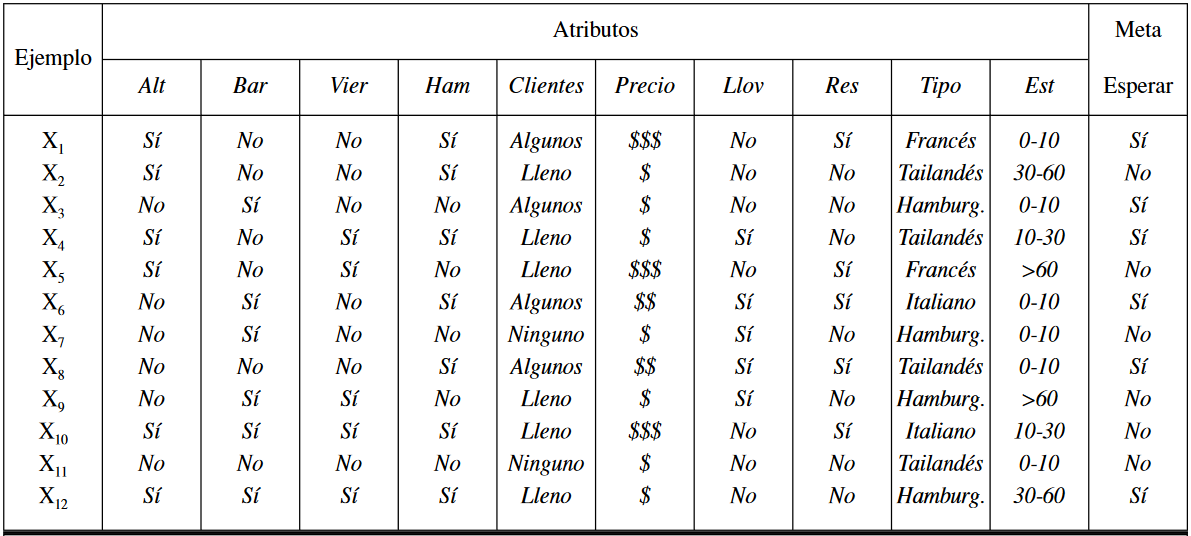
\includegraphics[width=\textwidth]{EjemploDT.png}
			\caption{Ejemplos para el dominio del restaurante}	
		\end{figure}
		Donde los ejemplos positivos son aquellos en los que la meta \(Esperar\) es verdadera, y los ejemplos negativos en los que es falsa. El conjunto de ejemplos completo se denomina \emph{conjunto de entrenamiento.}
		
		Esta definición de ejemplo no es la adecuada para este capítulo ya que aquí trabajamos con lógica de predicados, debído a esto en lugar de trabajar con un vector de atributos \(X\), nuestra entrada será una sentencia, donde los atributos se convertirán en predicados unarios, debido a esto ya no podemos pensar en nuestra entrada como ventor \(X\) más bien como una sentencia a la cual referenciaremos con \(E_{i}\) (entrada). Generalizando el ejemplo \(i\)-ésimo \(X_{i}\). Por ejemplo en el cuadro anterior, el primer ejemplo se describe a través de la sentencia:
			\[E_{1}:=Alternativa(X_{1}) \land \neg Bar(X_{1}) \land \neg Vier/Sab(X_{1}) \land Hambriento(X_{1}) \land ... \]
		
		\(D_{i}(X_{i})\) es una expresión cualquiera con unico argumento o aridad uno que representará el argumento de la entrada \(E_{i}\). El valor de salida del objeto \(E_{i}\) puede ser entedida como: La clasificación del objeto dada por la sentencia
			\[Esperar(X_{1})\]
			
		\(Q(X_{i})\) es una la notación genérica si el ejemplo es positivo, y \(\neg Q(X_{i})\) si el ejemplo es negativo. Esta notación generica es una sentencia que representa la salida del objeto \(E_{i}\) o mejor definida sentencia de clasificación o descripción. El conjunto completo de entrenamiento es la conjunción de todas las sentencias de descripción y clasificación.
		
		\textbf{Aprendizaje inductivo en el marco lógico} consiste en encontrar una expresión lógica equivalente al predicado meta \(Q\) con el objetivo de clasificar correctamente los ejemplos. Por \textbf{expresión lógica equivalente} al predicado meta \(Q\) nos referimos a una relación binaria a través del conectivo lógico de la doble implicación (\(\iff\)), esta relación no marca una relación fuerte que el lógica se denomina equivalente ya que si el antecedente es falso entonces el consecuente también es falso, y si el consecuente es verdadero el consecuente también los sera, es decir ambos tienen el mismo valor lógico. Por \textbf{clasificar correctamente los ejemplos} nos referimos a que dadas las entradas o sentencias \(E_{1}, E_{2},..,E_{i}\) la expresión econtrada debe darnos las salidas \(Q_{1},Q_{2},..,Q_{i}\). Cada \textbf{hipótesis} propone una expresión, que denominaremos una \textbf{definición candidata} del predicado meta. Usando \(C_{i}\) para representar la definición candidata, cada hipótesis \(h_{i}\) es una sentencia de la forma \(\forall Q(x) \iff C_{i}(x)\). En este punto conviene \emph{``separarnos''} un poco de la visión de función en la que veíamos nuestro formulación del aprendizaje y cabe centrarnos en la visión lógica, donde las entradas o \(E_{i}\), son sentencias que se tomarán como premisas verdaderas y nos servirán como base de conocimiento. 
		\begin{center}
			\textbf{Ejemplo:} Una hipótesis \(h_{r}\) pronene una definición candidata \(C_{r}\), la cual en lenguaje natural es: un predicado meta es verdadero para un objeto si y sólo si se alcanza una de las ramas que llevan a \emph{verdadero}. Formilazando esto en lógica:
		\end{center}
		\begin{figure}[h]
			\centering
			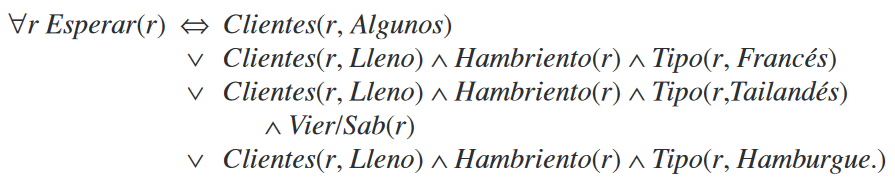
\includegraphics[width=0.9\textwidth]{candidateDefinition.png}
		\end{figure}

		Cada hipótesis predice que un cierto conjunto de ejemplos, es decir aquellos que satisfacen\footnote{Por satisfacer entendemos toda formula que es verdedara.} su definición candidata, serán ejemplos del predicado meta, en otras palabras toda \(C_{j}(x)\) de una hipotesis \(h_{j}\) que sea verdadero y que pertenezca al conjunto de ejemplos. Este conjunto se denomina \textbf{extensión} del predicado. Dos hipótesis con distintas extensiones son inconsistentes entre sí (\(\iff\)). Si tienen la misma extensión, son lógicamente equivalentes.
		\begin{figure}[hbt!]		
			\centering
			\import{img/}{set.pdf_tex}
			\caption{$\mathcal{A}$=Todas las posibles predicciones de $C_{j}$. $\mathcal{B}$=Predicciones positivas de $C_{j}$. $\mathcal{C}$= Predicciones de $C_{j}$ que forman parte del conjunto de ejemplos.}
			\label{fig: set_output}
		\end{figure}
		
		El espacio de hipótesis \(H\) es el conjunto de todas las hipótesis \(h_{1},..,h_{n}\) que el algoritmo de aprendizaje está diseñado para considerar. Se supone que el algoritmos de aprendizaje considera que una de la hipótesis es correcta:
		$$h_{1} \lor h_{2} \lor h_{3}\lor ... \lor h_{n}$$
		
		Podemos ir excluyendo las hipotesis que no son \emph{consistentes}, la no consitencia para un ejemplo puede ocurrir de dos formas:
		
		\begin{itemize}
			\item Un ejemplo puede ser \textbf{falso negativo} para la hipótesis, si la hipótesis afirma que debe ser negativo pero en realidad es positivo.\\
			\item Un ejemplo puede ser un \textbf{falso positivo} para la hipótesis, si la hipótesis afirma quedebe ser positivo pero en realidad es negativo.
		\end{itemize}
		
		Entonces un ejemplo puede ser incosistente con una hipotesis, podemos aprovechar esto para ir eliminando una o más hipotesis.
		 
		 Por lo tanto, podemos caracterizar el aprendizaje inductivo en un marco lógico como un proceso de eliminación gradual de las hipótesis que son incosistentes con los ejemplos, reduciendo así las probabilidades. Sin embargo pueden existir espacios de hipotesis enormes e incluso infinitos por eso describimos dos enfoques que encuentran hipótesis lógicamente con mucho menos esfuerzo.
		 
		 \subsection{Búsqueda mejor-hipótesis-actual}
			La idea de la búsqueda mejor-hipotesis-actual es mantener una única hipótesis, y ajustarla cuando llegan nuevos ejemplos para que se mantenga la consistencia.
			
			Supongamos que tenemos una hipótesis \(h_{r}\) cualquiera, y hasta el momento todos los ejemplos son consistentes. Donde el rectangulo es la extesión de \(h_{r}\). Entonces surge un ejemplo falso negativo, por lo tanto ese ejemplo debería formar parte de la extensión. La extensión debe \emph{aumentarse} e incluirlo. A esto se denomina \textbf{generalización}. Sin embargo surge otro ejemplo falso positivo, por lo tanto ese ejemplo no debería formar parte de la extensión. La extensión debe \emph{reducirse} y excluirla. A esto se denomina \textbf{especialización}.
				\begin{figure}[h]
					\centering
					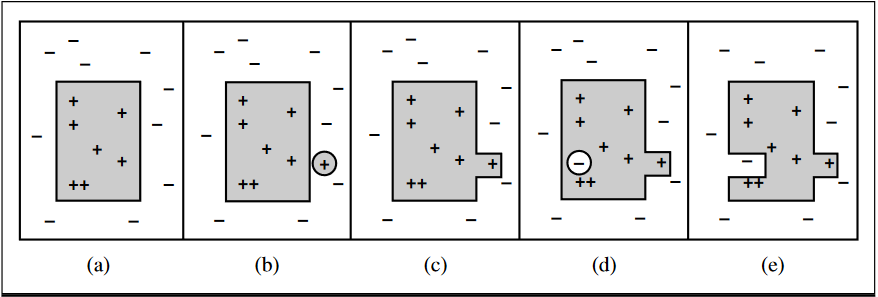
\includegraphics[width=0.9\textwidth]{SG.png}
				\end{figure}
			Ya en el algoritmo, tanto la espeficicación y generalización deben comprobar la consistencia con el resto de ejemplos.
			
				\begin{figure}[h]
					\centering
					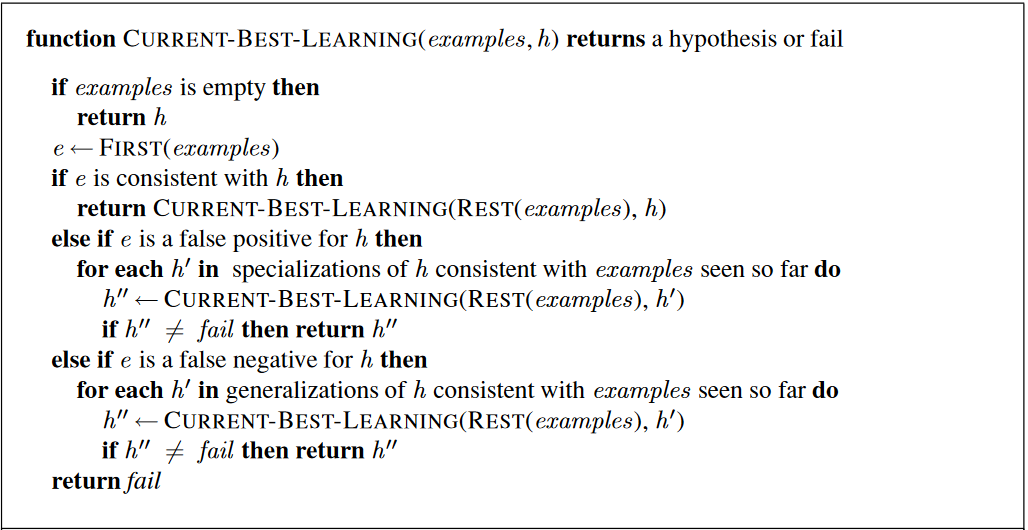
\includegraphics[width=0.9\textwidth]{BMHA_algorithm.png}
					\caption{Busca una hipótesis consistente que ajuste todos los ejemplos.}%pendiente.
				\end{figure}
			Entonces definimos la generalización y especialización como operaciones que cambian la \emph{extension} de nuestra hipótesis. Ahora necesitamos implementar operaciones sintácticas de manera exacta que modifiquen la definición candidata (\(C_{j}\)) asociada con la hipotesis. Esto se realiza observando que la generalización y la especialización son \textbf{realciones lógicas entre hipótesis}. Si la hipótesis $h_{1}$, con la definición $C_{1}$, es una generalización de la hipótesis $h_{2}$ con la definición $C_{2}$, entonces debemos tener
				$$\forall x C_{2}(x) \Rightarrow C_{1}(x)$$
			Por lo tanto, para construir una generalización de $h_{2}$, necesitamos la definición $C_{1}$ que sea una implicación lógica de $C_{2}$. 
			
			Existen varias operaciones de gerneralización, pero el que usaremos será la \textbf{omisión de condiciones} (dropping conditions). Para especializar podemos \textbf{agregar condiciones} o \textbf{elimanar disyunciones} de una definición disyuntiva.
			
			\textbf{Ejemplo:} Usando la tabla de la figura 1, iremos construyendo nuestra hipotesis.
			\begin{itemize}
				\item El primer ejemplo $X_{1}$ es positivo. $Alternativa(X_{1})$ es verdadero, así que la hipótesis inicial será
					$$h_{1}: \forall x Esperar(x) \Leftrightarrow Alternativa(x)$$
				\item El segundo ejemplo $X_{2}$ es negativo. $h_{1}$ lo predice como positivo, así que es un falso positivo. Por ello, tenemos que especializar $h_{1}$. Se puede hacer añadiendo una condición extra que rehace $X_{2}$. Una posibilidad es
					$$h_{2}: \forall x Esperar(x) \Leftrightarrow Alternativa(x) \land Clientes(x, Algunos)$$
				\item  El tercer ejemplo $X_{3}$ es positivo. $h_{2}$ lo predice como negativo, luego es un falso negativo. Por ello, necesitamos generalizar $h_{2}$. Eliminamos la condición Alternativa, resultando
					$$h_{3}:\forall x Esperar(x) \Leftrightarrow Clientes(x, Algunos)$$
				\item El cuarto ejemplo $X_{4}$ es positivo. $h_{3}$ lo predice como negativo, luego es un falso negativo. Por ello, necesitamos generalizar. No podemos eliminar la condición de $Clientes$, ya que obtendríamos una hipótesis que incluye a todos los ejemplos,que sería inconsistente con $X_{2}$. Una posibilidad es añadir una disyunción:
					$$h_{4}:\forall x Esperar(x) \Leftrightarrow Clientes(x, Algunos)\lor (Clientes(x, Lleno) \land Vier/Sab(x))$$
			\end{itemize}
				
				La hipótesis ya está comenzando a parecer razonable. Obviamente, existen otras posibilidades consistentes con los cuatro primeros ejemplos; aquí están otras dos:
					$$h_{4}':\forall x Esperar(x) \Leftrightarrow \neg TiempoEsperaEstimado(x, 30-60)$$
					$$h_{4}'':\forall x Esperar(x) \Leftrightarrow Clientes(x, Algunos)$$ 
					$$\lor (Clientes(x, Lleno) \land TiempoEsperaEstimado(x, 10-30))$$
			Este tipo de algoritmo es muy caro computacionalmente debido al \emph{backtraking}, se dice que es doblemente exponencial.
			
		%\subsection{Búsqueda de mínimo compromiso}
			
%%%%%%%%%%%%%%%%%%%%%%%%%%%%%%%%%%%%%%
	\section{Conocimiento en el aprendizaje}
	 	\subsection{Aprendizaje con conocimiento básico}
	 		El aprendizaje inductivo se basa en el descubrimiento de patrones a partir de ejemplos.
			
			El conocimiento a priori es aquel que, en algún sentido importante, es independiente de la experiencia.Para entender el papel del conocimiento a priori, necesitamos hablar de las relaciones lógicas entre hipótesis, descripciones de ejemplos y clasificaciones.
			
			\textbf{Descripciones:} Conjunción de todas las descripciones de los ejemplos del conjunto de entrenamiento.
			
			\textbf{Clasificaciones:} Conjunción de todas las clasificaciones de los ejemplos.
De este modo, las Hipótesis que ``explican las observaciones'' deben satisfacer la siguiente propiedad:
				
				\begin{figure}[h]
					\centering
					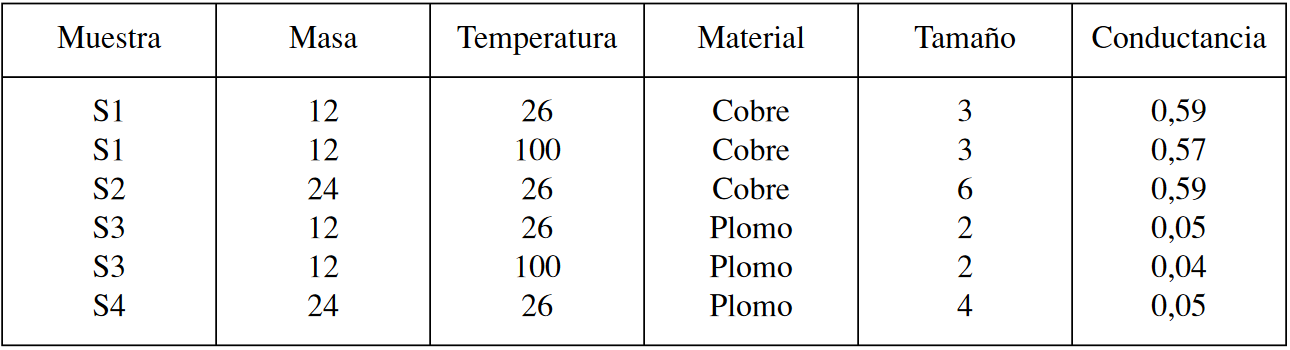
\includegraphics[width=0.6\textwidth]{./section2/fig1.png}
				\end{figure}
			
			Esta relación se denomina restricción, donde Hipótesis es lo<<desconocido>>.  El objetivo del aprendizaje inductivo puro es resolver esta restricción, donde Hipótesis se obtiene a partir de algún espacio de hipótesis predefinido.
			
			Para construir un \emph{agente de aprendizaje autónomo que utilice conocimiento básico}, el agente debe contar con algún método para obtener el conocimiento básico, para que este conocimiento se pueda utilizar en los nuevos episodios de aprendizaje. Este método también debe ser en sí mismo un proceso de aprendizaje, la historia de la vida del agente estará caracterizada por un desarrollo acumulativo o incremental.
				\begin{figure}[h]
					\centering
					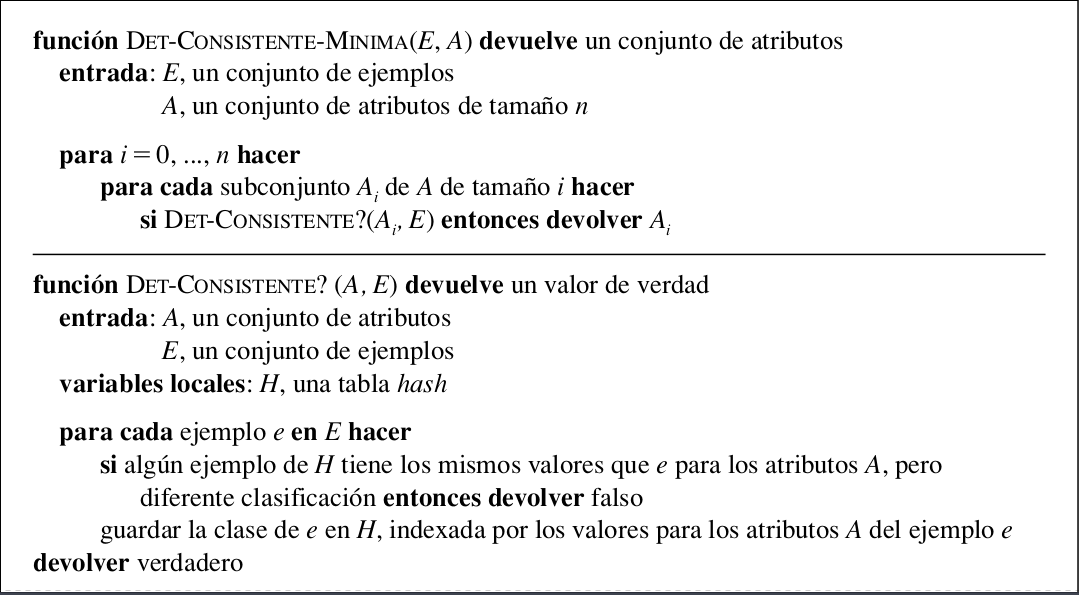
\includegraphics[width=0.85\textwidth]{./section2/fig2.png}
				\end{figure}
		\subsection{Ejemplos de aprendiaje con conocimiento básico}
			\subsubsection{Aprendizaje basado en explicaciones (EBL)}
			Ejemplo: Un hombre primitivo, está asando un lagarto en una vara. Es observado por una multitud asombrada de sus contemporáneos menos intelectuales, quienes han venido utilizando sus manos desnudas para mantener sus provisiones sobre el fuego. Esta instructiva experiencia es suficiente para convencer a los observadores de un principio general para cocinar sin dolor.
			
			Tipo de restricción: El hombre primitivo generaliza explicando el éxito de la vara: ésta soporta al lagarto, manteniendo así la mano lejos del fuego. A partir de esta explicación, infiere una \emph{regla general}: que cualquier objeto largo, rígido y puntiagudo sirve para asar alimentos pequeños y ligeros.
			
			Este tipo de proceso de generalización es denominado aprendizaje basado en explicaciones, o EBL (Explanation Based Learning). La regla general se deduce lógicamente del conocimiento básico que posee el hombre primitivo. Por lo tanto, las restricciones que se satisfacen por el EBL son las siguientes:
				\begin{figure}[h]
					\centering
					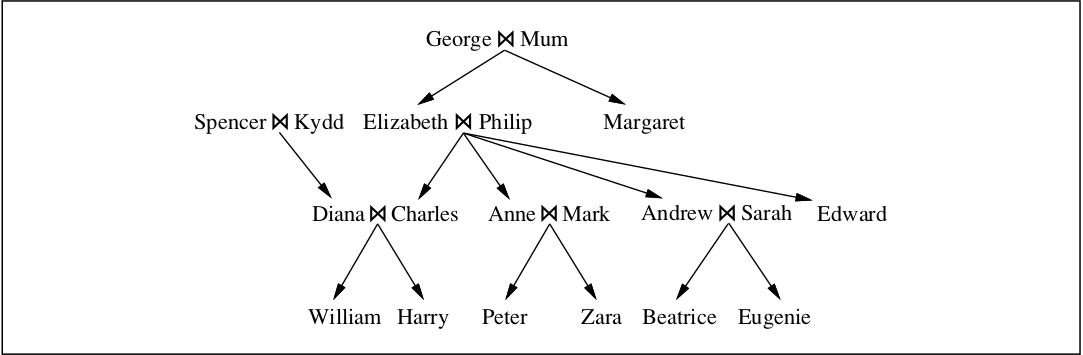
\includegraphics[width=0.6\textwidth]{./section2/fig3.png}
				\end{figure}
			
			EBL necesita que exista suficiente conocimiento básico como para explicar la Hipótesis, que en realidad explica las observaciones, por tanto, realmente el agente no aprende nada nuevo del ejemplo. El agente podría haber derivado el ejemplo de lo que ya sabía, aunque esto requiriera una cantidad muy elevada de computación. EBL no se considera como un método para convertir los primeros principios de las teorías en conocimiento útil de propósito específico.
			\subsubsection{Aprendizaje basado en Relevancia (RBL)}
			Ejemplo: Un turista va a Brasil y conoce a su primera persona brasileña. Al escucharle hablar en portugués, inmediatamente concluirá que los brasileños hablan en portugués, aunque al descubrir que su nombre es Fernando no concluirá que todos los brasileños se llaman Fernando.
			
			En este caso, el conocimiento a priori relevante es que, en cualquier país, la mayoría de la gente habla el mismo idioma; por otro lado, no se asume que Fernando sea el nombre de todos los brasileños, porque este tipo de regularidad no se verifica para los nombres.

			En este caso, el Conocimiento Básico a priori se refiere a la relevancia que tiene un conjunto de características sobre el predicado meta. Este conocimiento, junto con las observaciones, permite al agente inferir una nueva regla general que explica las observaciones:
				\begin{figure}[h]
					\centering
					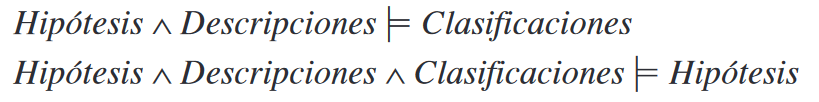
\includegraphics[width=0.8\textwidth]{./section2/fig4.png}
				\end{figure}
			
			Como el RBL no hace uso del contenido de las observaciones, no produce hipótesis que vayan más allá del contenido lógico del conocimiento básico y de las observaciones. Es un método de aprendizaje deductivo, y por sí mismo no puede justificar la creación de nuevo conocimiento sin un conocimiento inicial de partida.
			
			\subsubsection{Aprendizaje inductivo basado en el conocimiento (Algoritmo KBIL)}
			\textbf{Ejemplo:} Un estudiante de Medicina sabe realizar diagnósticos sofisticados, pero es ignorante respecto a farmacología, está observando la consulta entre un paciente y un experto. Después de una serie de preguntas y respuestas, el experto dice al paciente que tome un determinado antibiótico. El estudiante de medicina inferirá la regla general sobre qué antibiótico particular es efectivo para un tipo de infección determinado.
			
			Se asume que el conocimiento a priori del estudiante es suficiente para inferir la enfermedad (D) del paciente a partir de los síntomas. Sin embargo, esto no es suficiente para explicar el hecho de que el doctor prescribe una medicina concreta (M) El estudiante necesita obtener otra regla: que M, generalmente, es una medicina efectiva contra la enfermedad D. Dada esta regla, y el conocimiento a priori con el que cuenta el estudiante, éste puede explicar por qué el experto prescribe M en ese caso particular. Podemos generalizar este ejemplo para proponer la restricción:
				\begin{figure}[h]
					\centering
					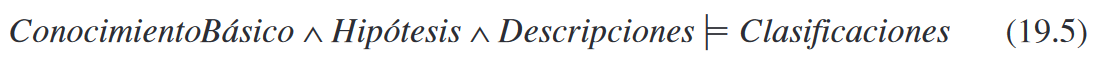
\includegraphics[width=1\textwidth]{./section2/fig5.png}
				\end{figure}
			
	 \section{Aprendizaje basado en explicaciones}
	 		El aprendizaje basado en explicaciones es un método para extraer reglas generales a partir de observaciones particulares.
	 			\begin{figure}[h]
					\centering
					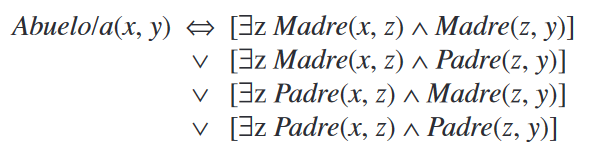
\includegraphics[width=0.8\textwidth]{./section2/fig6.png}
				\end{figure}
	 		Supongamos que estamos aprendiendo a integrar. Sabemos las reglas de integración, la tabla de integrales inmediatas y los métodos que podemos usar para resolverlas. Al principio, cuando nos dan una integral para resolver, vamos probando métodos hasta encontrar uno que nos de la solución de forma sencilla. Esto es, si decidimos aplicar un método y este nos lleva a una expresión más complicada, lo descartamos y probamos con otro. A medida que aumentamos nuestra experiencia en la resolución de integrales sabremos a simple vista" cuál es el método más apropiado para obtener la solución. Un método EBL puede asociarse a un sistema de resolución de problemas de manera que nos permitirá aprender reglas de control que mejorarán su eficiencia
	 			\begin{figure}[h]
					\centering
					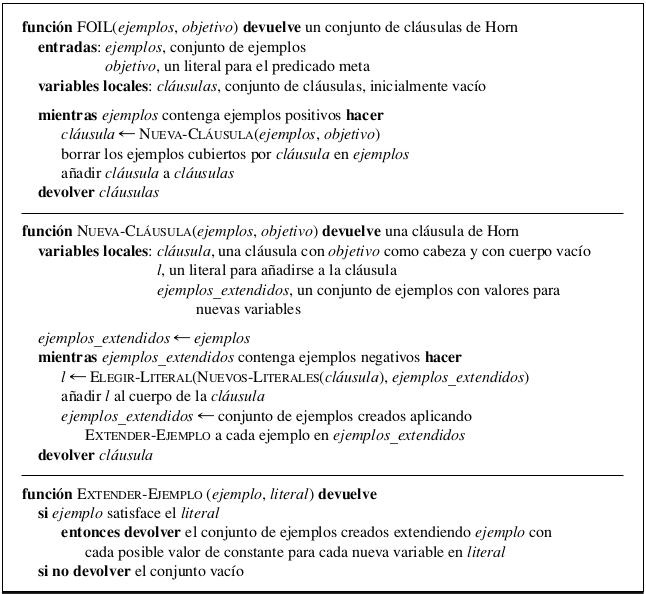
\includegraphics[width=0.8\textwidth]{./section2/fig7.png}
				\end{figure}
	 		\subsection{Técnicas de la memorización}
	 		La técnica de memorización ha sido extensamente utilizada en informática para acelerar los programas guardando los resultados de la computación. La idea básica de las funciones memo es acumular una base de datos de pares entrada/salida; cuando se hace una llamada a la función, ésta, en primer lugar, comprueba la base de datos para ver si se puede evitar que la resolución del problema parta de cero.
	 		
	 		\subsection{Extracción de reglas generales a partir de ejemplos:}
			La idea en la que se basa EBL consiste en construir, en primer lugar, una explicación de la observación, utilizando conocimiento a priori, y posteriormente, establecer una definición de la clase de casos para los que se puede utilizar la misma estructura de explicación. Esta definición proporciona las bases para una regla que cubra todos los casos en la clase. La ``explicación'' puede ser una prueba lógica, aunque de forma más general, puede ser cualquier proceso de razonamiento o de resolución de problemas cuyos pasos estén bien definidos. La clave es ser capaz de identificar las condiciones necesarias para que los mismos pasos se puedan aplicar a otro caso.
			
			\subsection{Encadenamiento hacia atrás}
			El proceso de desarrollo de un Sistema basado en encadenamiento hacia atrás está dado de la siguiente manera:

			\begin{itemize}
				\item Se comienza con una meta para probar\\
				\item Se inspecciona la memoria de trabajo para ver si la meta ha sido     previamente probada\\
				\item En caso de que no se haya probado, el sistema busca en sus reglas para ver si     una o más tienen esta meta en su parte del THEN, este tipo de regla     es llamada regla meta.\\
				\item El sistema ve si las premisas de las reglas meta están listadas en la memoria     de trabajo, las premisas no listadas se tornan nuevas metas o     subtemas para ser probadas.\\
				\item Este proceso continúa de manera recursiva hasta que el sistema encuentra una     premisa que no es soportada por ninguna regla, llamada primitiva     (premisa de una regla que no es concluida por ninguna regla)\\
				\item Cuando una primitiva es encontrada, el sistema pregunta al usuario información     acerca de esta primitiva, entonces el sistema usa esta información     para ayudar a probar los subtemas y la meta original\\
			\end{itemize}	
				\begin{figure}[h]
					\centering
					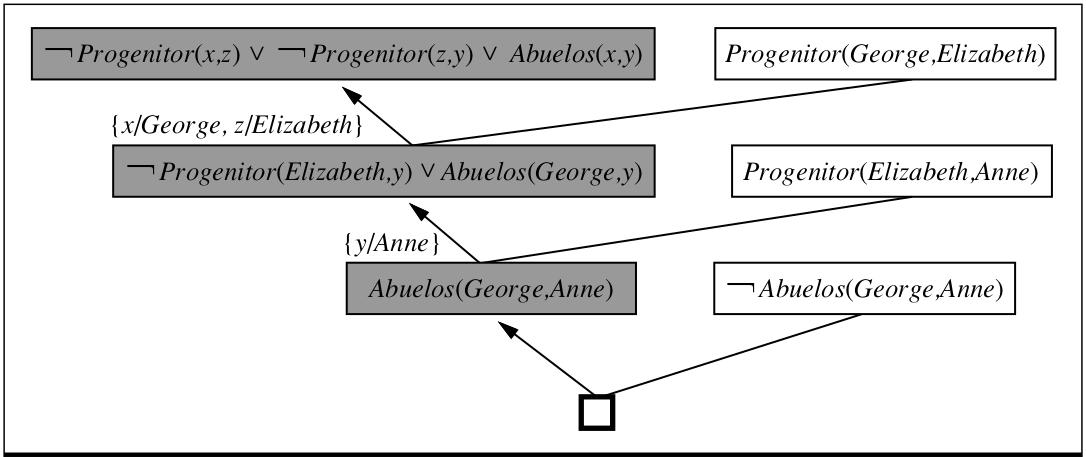
\includegraphics[width=0.6\textwidth]{./section2/fig8.png}
				\end{figure}
			
			En el encadenamiento hacia atrás, el orden a probar la hipótesis h deberá de probarse al menos una de las hipótesis intermedias. Se observa que el diagrama, en este caso se describe como un diagrama AND/OR para indicar que en algún caso, tal como h2 todas las hipótesis de nivel inferior deben estar presentes para sostener h2.
	
			En otros casos, tal como la hipótesis de nivel superior h solo es necesario una hipótesis de nivel inferior para que se verifique.En el encadenamiento hacia atrás, el sistema, por lo general, obtendrá evidencia del usuario, con el fin de probar o no la hipótesis, lo que contrasta con el sistema de encadenamiento hacia adelante, en el que todos los hechos relevantes se conocen por lo general con antelación.
			\subsubsection{Ejemplo del ecadenamiento hacia atrás}
			Supongamos que un paciente va al doctor, el doctor luego de escuchar el problema del paciente creé que tiene una infección de garganta. Ahora bien veremos como un sistema experto basado en reglas de encadenamiento hacia atrás puede solucionar este problema.
			
			\subsection{Proceso básico de EBL}
			El proceso básico de EBL funciona de la siguiente forma:
				\begin{enumerate}
						\item Dado un ejemplo, se construye una prueba para el predicado meta que se aplica al ejemplo, utilizando el conocimiento básico disponible.\\
						  \item En paralelo, se construye un árbol de prueba generalizado para la meta variabilizada, utilizando los mismos pasos de inferencia que en la prueba original.\\
						  \item Se construye una nueva regla cuya parte izquierda está formada por las hojas del árbol de prueba y cuya parte derecha es la meta variabilizada (después de aplicar las asignaciones necesarias de la prueba generalizada).\\
						  \item Se eliminan todas las condiciones que son verdaderas independientemente de los valores de las variables de la meta.\\
				\end{enumerate}

	 \section{Aprendizaje basado en información relevante}
	
	 \section{Programación lógica inductiva}
	 
\end{document}
